\documentclass[tikz,convert={outfile=images/monad-unitality.svg,density=1000}]{standalone}
\usepackage[build={latexoptions={-output-directory=latex/svg}}]{standalone}
\begin{document}
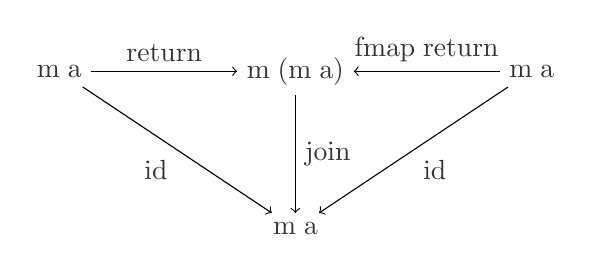
\begin{tikzpicture}
    \node (A) at (0,2) {\textcolor{black!80}{\(\mathrm{m\;a}\)}};
    \node (B) at (3,2) {\textcolor{black!80}{\(\mathrm{m\;(m\;a)}\)}};
    \node (C) at (6,2) {\textcolor{black!80}{\(\mathrm{m\;a}\)}};
    \node (D) at (3,0) {\textcolor{black!80}{\(\mathrm{m\;a}\)}};
    \draw [->] (A) -- node[above] {\textcolor{black!80}{\(\mathrm{return}\)}} (B); 
    \draw [->] (C) -- node[above] {\textcolor{black!80}{\(\mathrm{fmap\;return}\)}} (B);
    \draw [->] (B) -- node[right] {\textcolor{black!80}{\(\mathrm{join}\)}}  (D);
    \draw [->] (A) -- node[below left]  {\textcolor{black!80}{\(\mathrm{id}\)}} (D);
    \draw [->] (C) -- node[below right] {\textcolor{black!80}{\(\mathrm{id}\)}} (D);
\end{tikzpicture}
\end{document}
